% aeolian cheat sheet: two landscape A4 pages.  Build: make cheatsheet
% Every number here comes from lib/aeolian_ctl.h and lib/aeolian_harp.h
% (dial values printed from that code).
\documentclass{article}
\usepackage[a4paper,landscape,margin=6mm]{geometry}
\usepackage[T1]{fontenc}
\usepackage{lmodern}
\usepackage[default]{sourcesanspro}
\usepackage{amssymb}
\usepackage{amsmath}
\usepackage{tikz}
\usepackage[most]{tcolorbox}
\usepackage{array}
\usepackage{tabularx}
\pagestyle{empty}
\setlength{\parindent}{0pt}

\definecolor{ink}{RGB}{30,30,30}
\definecolor{snd}{RGB}{20,20,20}       % SOUND-page knob labels
\definecolor{fxc}{RGB}{30,90,170}      % FX-page knob labels
\definecolor{wndc}{RGB}{0,130,120}     % wind
\definecolor{strc}{RGB}{170,90,20}     % strings
\definecolor{wxc}{RGB}{150,60,170}     % weather
\definecolor{freec}{RGB}{170,170,170}  % unassigned
\definecolor{padc}{RGB}{120,170,230}

\newcommand{\FX}[1]{\textcolor{fxc}{#1}}
\newcommand{\WN}[1]{\textcolor{wndc}{#1}}
\newcommand{\ST}[1]{\textcolor{strc}{#1}}
\newcommand{\WX}[1]{\textcolor{wxc}{#1}}
\newcommand{\FR}[1]{\textcolor{freec}{#1}}
\newcommand{\cc}[1]{\textcolor{black!45}{\fontsize{4.6}{5}\selectfont #1}}

% knob: x, SOUND label (above), FX label (below)
\newcommand{\knob}[3]{%
  \draw[fill=black!8, draw=black!60, line width=0.4pt] (#1,62) circle (3.6);
  \draw[black!60, line width=0.5pt] (#1,62) -- ++(110:3.1);
  \node[font=\fontsize{5.6}{6.2}\selectfont\bfseries, text=snd, align=center] at (#1,69.4) {#2};
  \node[font=\fontsize{5.6}{6.2}\selectfont, text=fxc, align=center] at (#1,54.4) {#3};}
\newcommand{\pad}[3]{%
  \draw[rounded corners=0.8mm, fill=padc!35!white, draw=padc!80!black, line width=0.4pt]
    (36+#1*13.2, 21+#2*13.2) rectangle ++(12,12);
  \node[font=\fontsize{5.4}{6}\selectfont, text=ink, align=center, text width=11mm]
    at (36+#1*13.2+6, 21+#2*13.2+6) {#3};}
\newcommand{\fader}[3]{%
  \draw[fill=black!12, draw=black!50] (#1-0.7,26) rectangle (#1+0.7,52);
  \draw[fill=#3!60!white, draw=#3!70!black, rounded corners=0.4mm] (#1-2.6,36) rectangle (#1+2.6,40);
  \node[font=\fontsize{5.6}{6.2}\selectfont\bfseries, text=#3!70!black, align=center] at (#1,56) {#2};}
\newcommand{\btn}[5]{%
  \draw[rounded corners=0.6mm, fill=#4!25!white, draw=#4!70!black, line width=0.4pt]
    (#1-#5/2,#2-2.6) rectangle (#1+#5/2,#2+2.6);
  \node[font=\fontsize{4.9}{5.4}\selectfont, text=ink, align=center] at (#1,#2) {#3};}

\tcbset{card/.style={enhanced, colback=white, colframe=black!70, boxrule=0.5pt, arc=1.5mm,
    left=1.6mm, right=1.6mm, top=1.1mm, bottom=1.1mm, toptitle=0.6mm, bottomtitle=0.6mm,
    fonttitle=\bfseries\fontsize{8.6}{10}\selectfont, coltitle=white, colbacktitle=black!75,
    fontupper=\fontsize{7.1}{8.5}\selectfont, before skip=0mm, after skip=1.8mm}}
\newtcolorbox{card}[1]{card, title={#1}}
\newcolumntype{L}{>{\raggedright\arraybackslash}X}

\begin{document}

{\fontsize{16}{18}\selectfont\bfseries aeolian}\hspace{3mm}%
{\fontsize{9.5}{11}\selectfont Axoloti Core + Launchkey 49 MK3 (standalone mode) \textperiodcentered{}
a wind harp: eight strings, the wind plays them \textperiodcentered{} \texttt{patches/aeolian/aeolian\_v1.axp}}\hfill
{\fontsize{7}{8}\selectfont\color{black!55} v1.0 \textperiodcentered{} 2026-11-12 \textperiodcentered{} page 1 of 2}

\vspace{1.5mm}
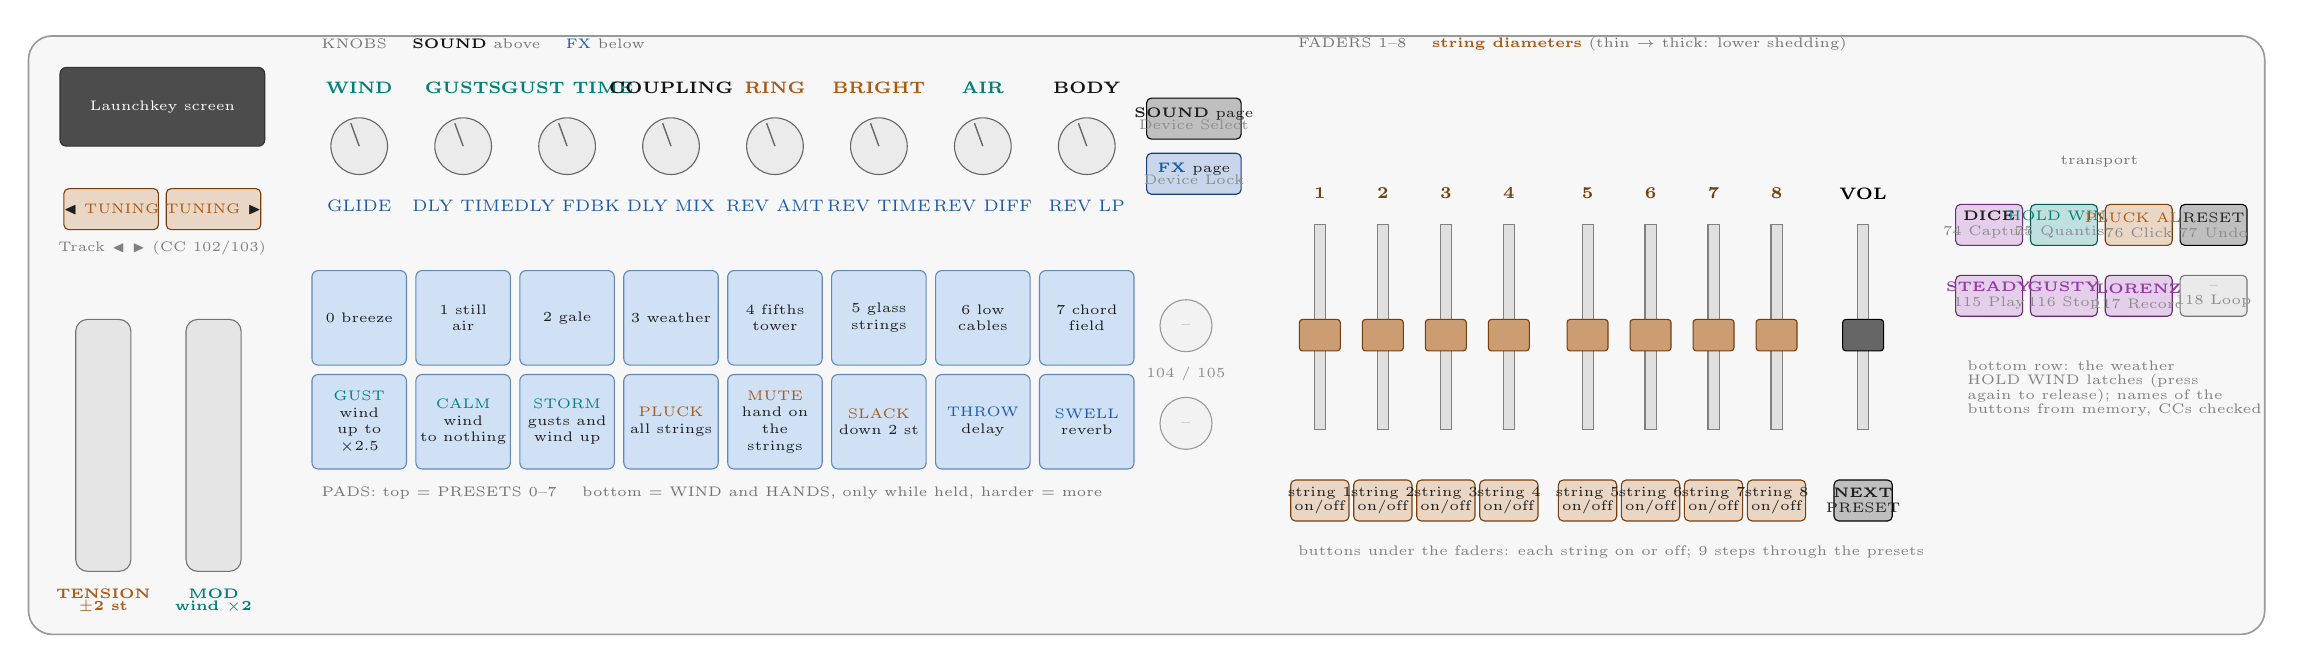
\begin{tikzpicture}[x=1mm,y=1mm]
  \draw[rounded corners=3mm, fill=black!3, draw=black!40, line width=0.6pt] (0,0) rectangle (284,76);

  % ---- left: screen, track buttons, wheels
  \draw[fill=black!70, draw=black!80, rounded corners=0.8mm] (4,62) rectangle (30,72);
  \node[font=\fontsize{5}{6}\selectfont, text=white] at (17,67) {Launchkey screen};
  \btn{10.5}{54}{\(\blacktriangleleft\) \ST{TUNING}}{strc}{12}
  \btn{23.5}{54}{\ST{TUNING} \(\blacktriangleright\)}{strc}{12}
  \node[font=\fontsize{4.6}{5}\selectfont, text=black!50] at (17,49) {Track \(\blacktriangleleft\) \(\blacktriangleright\) (CC 102/103)};
  \draw[rounded corners=1.5mm, fill=black!10, draw=black!55] (6,8) rectangle (13,40);
  \draw[rounded corners=1.5mm, fill=black!10, draw=black!55] (20,8) rectangle (27,40);
  \node[font=\fontsize{5.4}{6}\selectfont\bfseries, align=center, text=strc] at (9.5,4.2) {TENSION\\[-0.6mm]\(\pm\)2 st};
  \node[font=\fontsize{5.4}{6}\selectfont\bfseries, align=center, text=wndc] at (23.5,4.2) {MOD\\[-0.6mm]wind \(\times\)2};

  % ---- knobs: SOUND (top) / FX (blue, below)
  \node[font=\fontsize{5}{6}\selectfont, text=black!55, anchor=west] at (36,75) {KNOBS \quad
     \textbf{\textcolor{snd}{SOUND}} above \quad \FX{FX} below};
  \knob{42}{\WN{WIND}}{\FX{GLIDE}}
  \knob{55.2}{\WN{GUSTS}}{\FX{DLY TIME}}
  \knob{68.4}{\WN{GUST TIME}}{\FX{DLY FDBK}}
  \knob{81.6}{COUPLING}{\FX{DLY MIX}}
  \knob{94.8}{\ST{RING}}{\FX{REV AMT}}
  \knob{108}{\ST{BRIGHT}}{\FX{REV TIME}}
  \knob{121.2}{\WN{AIR}}{\FX{REV DIFF}}
  \knob{134.4}{BODY}{\FX{REV LP}}
  \btn{148}{65.5}{\textbf{SOUND} page\\[-0.4mm]\cc{Device Select}}{black}{12}
  \btn{148}{58.5}{\textbf{\FX{FX}} page\\[-0.4mm]\cc{Device Lock}}{fxc}{12}

  % ---- pads
  \pad{0}{1}{0 breeze} \pad{1}{1}{1 still\\air} \pad{2}{1}{2 gale} \pad{3}{1}{3 weather}
  \pad{4}{1}{4 fifths\\tower} \pad{5}{1}{5 glass\\strings} \pad{6}{1}{6 low\\cables} \pad{7}{1}{7 chord\\field}
  \pad{0}{0}{\WN{GUST}\\wind\\up to \(\times\)2.5} \pad{1}{0}{\WN{CALM}\\wind\\to nothing} \pad{2}{0}{\WN{STORM}\\gusts and\\wind up}
  \pad{3}{0}{\ST{PLUCK}\\all strings} \pad{4}{0}{\ST{MUTE}\\hand on\\the strings} \pad{5}{0}{\ST{SLACK}\\down 2 st}
  \pad{6}{0}{\FX{THROW}\\delay} \pad{7}{0}{\FX{SWELL}\\reverb}
  \node[font=\fontsize{5}{6}\selectfont, text=black!55, anchor=west] at (36,18) {PADS: top = PRESETS 0--7 \quad bottom = WIND and HANDS, only while held, harder = more};
  \draw[fill=black!5, draw=black!40] (147,39.2) circle (3.3);
  \draw[fill=black!5, draw=black!40] (147,26.8) circle (3.3);
  \node[font=\fontsize{4.6}{5}\selectfont, text=freec] at (147,39.2) {--};
  \node[font=\fontsize{4.6}{5}\selectfont, text=freec] at (147,26.8) {--};
  \node[font=\fontsize{4.2}{5}\selectfont, text=black!45] at (147,33) {104 / 105};

  % ---- faders: string diameters
  \node[font=\fontsize{5}{6}\selectfont, text=black!55, anchor=west] at (160,75) {FADERS 1--8 \quad
     \ST{\textbf{string diameters}} (thin \(\to\) thick: lower shedding)};
  \fader{164}{1}{strc} \fader{172}{2}{strc} \fader{180}{3}{strc} \fader{188}{4}{strc}
  \fader{198}{5}{strc} \fader{206}{6}{strc} \fader{214}{7}{strc} \fader{222}{8}{strc}
  \fader{233}{VOL}{black}
  \btn{164}{17}{string 1\\on/off}{strc}{7.4}
  \btn{172}{17}{string 2\\on/off}{strc}{7.4}
  \btn{180}{17}{string 3\\on/off}{strc}{7.4}
  \btn{188}{17}{string 4\\on/off}{strc}{7.4}
  \btn{198}{17}{string 5\\on/off}{strc}{7.4}
  \btn{206}{17}{string 6\\on/off}{strc}{7.4}
  \btn{214}{17}{string 7\\on/off}{strc}{7.4}
  \btn{222}{17}{string 8\\on/off}{strc}{7.4}
  \btn{233}{17}{\textbf{NEXT}\\PRESET}{black}{7.4}
  \node[font=\fontsize{4.6}{5}\selectfont, text=black!50, anchor=west] at (160,10.5) {buttons under the faders: each string on or off; 9 steps through the presets};

  % ---- transport (ch 16)
  \node[font=\fontsize{5}{6}\selectfont, text=black!55] at (263,60) {transport};
  \btn{249}{52}{\textbf{DICE}\\\cc{74 Capture}}{wxc}{8.5}
  \btn{258.5}{52}{\WN{HOLD WIND}\\\cc{75 Quantise}}{wndc}{8.5}
  \btn{268}{52}{\ST{PLUCK ALL}\\\cc{76 Click}}{strc}{8.5}
  \btn{277.5}{52}{RESET\\\cc{77 Undo}}{black}{8.5}
  \btn{249}{43}{\WX{\textbf{STEADY}}\\\cc{115 Play}}{wxc}{8.5}
  \btn{258.5}{43}{\WX{\textbf{GUSTY}}\\\cc{116 Stop}}{wxc}{8.5}
  \btn{268}{43}{\WX{\textbf{LORENZ}}\\\cc{117 Record}}{wxc}{8.5}
  \btn{277.5}{43}{\FR{--}\\\cc{118 Loop}}{freec}{8.5}
  \node[font=\fontsize{4.6}{5.2}\selectfont, text=black!50, align=left, anchor=north west] at (245,36)
     {bottom row: the weather\\HOLD WIND latches (press\\again to release); names of the\\buttons from memory, CCs checked};
\end{tikzpicture}

\vspace{1.2mm}
\begin{minipage}[t]{80mm}\vspace{0pt}
\begin{card}{How it sounds}
Eight strings in the wind. Wind across a string sheds vortices at the Strouhal frequency
\(f = 0.2\,U/d\) (wind \(U\), diameter \(d\)). When \(f\) comes near one of the string's harmonics, the wake
\emph{locks in} and that harmonic sings; as the wind changes, harmonics bloom, fade and hop. An aeolian harp
mostly sings upper harmonics, rarely the fundamental. Nothing sounds without wind (or a pluck).\\[0.4mm]
\WN{WIND} up or thinner strings (faders down) \(\to\) higher harmonics. \textbf{COUPLING} sets how
strongly a harmonic holds on: low, harmonics swell as the wind passes them; high, a harmonic holds over a
wide range of wind and then jumps.
\end{card}
\begin{card}{Keys tune the harp (they do not play notes)}
\fontsize{6.8}{8.1}\selectfont
The last key is the root (raised to A1 at least); a key also plucks the strings it retunes, by velocity.
Releasing a key changes nothing: the harp keeps its tuning. Retuning glides (GLIDE, FX page).
\begin{tabularx}{\linewidth}{@{}l L@{}}
\ST{\textbf{UNISON}} & every string on the root, a few cents apart: as an aeolian harp is strung \\
\ST{\textbf{HARMONIC}} & the root's harmonic series 1--8 (just intonation) \\
\ST{\textbf{FIFTHS}} & root, 5th, octave, 12th, 2 octaves, 19th, an octave and a 4th below \\
\ST{\textbf{CHORD}} & the last eight keys (newest first), repeated an octave up \\
\end{tabularx}
\end{card}
\end{minipage}\hfill
\begin{minipage}[t]{70mm}\vspace{0pt}
\begin{card}{SOUND knobs}
\fontsize{6.8}{8.1}\selectfont
\begin{tabularx}{\linewidth}{@{}l L@{}}
\WN{\textbf{WIND}} & mean wind 0.5 -- 15 m/s \\
\WN{\textbf{GUSTS}} & gust size, 0 -- 60\,\% of the wind \\
\WN{\textbf{GUST TIME}} & how long a gust lasts, 0.2 -- 10 s (LORENZ: how fast the weather turns) \\
\textbf{COUPLING} & lock-in strength (wake \(\leftrightarrow\) string) \\
\ST{\textbf{RING}} & how long a string rings, 0.3 -- 18 s \\
\ST{\textbf{BRIGHT}} & how long the high harmonics ring, from 2\,\% of RING to all of it \\
\WN{\textbf{AIR}} & wind noise on the strings \\
\textbf{BODY} & the sound box: dry strings \(\to\) resonant box \\
\end{tabularx}
\end{card}
\begin{card}{Weather (Play / Stop / Record)}
\WX{\textbf{STEADY}}: the wind as set. \WX{\textbf{GUSTY}}: random gusts (size GUSTS, length GUST TIME).
\WX{\textbf{LORENZ}}: the wind follows the Lorenz system (a model of convection): it swings between two moods
and never repeats. Each string also sees a little turbulence of its own, so they never lock alike.
\end{card}
\end{minipage}\hfill
\begin{minipage}[t]{62mm}\vspace{0pt}
\begin{card}{Pads}
\textbf{Top} = presets 0--7. \textbf{Bottom}, while held; strike velocity, then pressure, sets the amount:
\fontsize{6.6}{7.9}\selectfont
\begin{tabularx}{\linewidth}{@{}l L@{}}
\WN{GUST} & more wind, up to \(\times\)2.5 \\
\WN{CALM} & the wind dies down to nothing \\
\WN{STORM} & bigger gusts, wind \(\times\)1.6 \\
\ST{PLUCK} & pluck every string (velocity) \\
\ST{MUTE} & a hand on the strings \\
\ST{SLACK} & strings down, up to 2 st \\
\FX{THROW / SWELL} & delay throw / reverb swell \\
\end{tabularx}
\end{card}
\begin{card}{Wheels and transport}
MOD: more wind (up to \(\times\)2). Pitch bend: string tension \(\pm\)2 st. HOLD WIND (Quantise) freezes the wind
where it is. PLUCK ALL (Click). DICE (Capture MIDI) rolls tuning, weather, SOUND page and gauges.
\end{card}
\end{minipage}\hfill
\begin{minipage}[t]{64mm}\vspace{0pt}
\begin{card}{The model}
\fontsize{6.6}{7.8}\selectfont
Each string: a digital waveguide, excited at a point; its loop tuned exactly (to 0.06 cent in the tests).
Each wake: a van der Pol oscillator (Facchinetti, de Langre \& Biolley 2004),
\[ \ddot q + \varepsilon\Omega(q^2-1)\dot q + \Omega^2 q = K\,\Omega^2\,v/L, \quad \Omega = 2\pi\,0.2\,U/d, \]
driving the string with the lift \(L\,q\), \(L \propto U^2 d\); \(v\) is the string's velocity at that point. Lock-in shows
hysteresis, as in vortex-induced vibration: rising wind holds a harmonic longer. Gusts: an
Ornstein--Uhlenbeck process; LORENZ: \(x\) of Lorenz-63. Code: \texttt{lib/aeolian\_harp.h}.
\end{card}
\begin{card}{Signal path and load}
8 strings \(\to\) sound box \(\to\) level control (slow; the wind swings 40 dB) \(\to\) stereo delay \(\to\)
Elements reverb \(\to\) VOL. DSP 75.5\,\%, constant (no voices to add); patch RAM 21 of 44 KB.
\end{card}
\end{minipage}

%======================================================================
\newpage
{\fontsize{16}{18}\selectfont\bfseries aeolian}\hspace{3mm}%
{\fontsize{9.5}{11}\selectfont presets, dial values, the Strouhal table, troubleshooting}\hfill
{\fontsize{7}{8}\selectfont\color{black!55} v1.0 \textperiodcentered{} page 2 of 2}

\vspace{1.5mm}
\begin{minipage}[t]{150mm}\vspace{0pt}
\begin{card}{Presets: top pads = 0--7; NEXT PRESET (fader button 9) steps; RESET (Undo) = 0 \quad\textmd{\fontsize{6.5}{7}\selectfont (chosen from the parameter meanings, not yet tuned by ear)}}
\fontsize{7.2}{8.7}\selectfont
\begin{tabularx}{\linewidth}{@{}>{\bfseries}l L@{}}
0 breeze & UNISON on A2, gusty 2.5 m/s, strings 0.4 -- 2.2 mm: the 2nd to 5th harmonics take turns. The power-on sound. \\
1 still air & HARMONIC series on D2, steady 1.4 m/s, rings 12 s: a slow, held chord of harmonics. \\
2 gale & UNISON on E2, 7.3 m/s with big, short gusts (0.6 s), more noise: high harmonics, restless. \\
3 weather & FIFTHS on G2, the Lorenz wind: calm and stormy spells that never repeat. \\
4 fifths tower & FIFTHS on C2, gentle gusts, strong lock-in, long ring: steady, overlapping fifths. \\
5 glass strings & UNISON on A3, thin strings (0.25 -- 0.6 mm), bright: the 7th to 10th harmonics, glassy. \\
6 low cables & HARMONIC on A1, thick strings (1.5 -- 3 mm), 6.4 m/s, dark, long ring, slow glide. \\
7 chord field & CHORD: play a few keys, the last eight stay strung; Lorenz wind. \\
\end{tabularx}\\[0.3mm]
A preset sets tuning, weather, root, both knob pages and the eight diameters; the volume stays.
\end{card}

\begin{card}{Sound design moves}
\fontsize{7.4}{9.0}\selectfont
\textbf{Harmonic glissando}: STEADY, COUPLING 3/4, sweep WIND (or the mod wheel) slowly: harmonics take over one
by one; sweep back down and they hold longer (hysteresis).\quad
\textbf{One string}: switch the others off (fader buttons) and play WIND against its diameter.\quad
\textbf{Gust gestures}: GUST and CALM pads with pressure.\quad
\textbf{Bowed metal}: AIR 0, RING full, BRIGHT 3/4, COUPLING full.\quad
\textbf{A chord in the wind}: CHORD, play it, then let the weather run.
\end{card}
\end{minipage}\hfill
\begin{minipage}[t]{128mm}\vspace{0pt}
\begin{card}{Where the values fall (knob turned \dots)}
\fontsize{7.5}{9.2}\selectfont
\setlength{\tabcolsep}{3pt}
\begin{tabular}{@{}l r r r r r@{}}
 & 0 & 1/4 & 1/2 & 3/4 & full \\ \hline
\WN{\textbf{WIND}} (m/s) & 0.5 & 1.2 & 2.8 & 6.4 & 15 \\
\WN{\textbf{GUSTS}} (of the wind) & 0 & 15\,\% & 30\,\% & 45\,\% & 60\,\% \\
\WN{\textbf{GUST TIME}} (s) & 0.2 & 0.54 & 1.4 & 3.7 & 10 \\
\textbf{COUPLING} \(K\) & 0.001 & 0.0024 & 0.0056 & 0.013 & 0.03 \\
\ST{\textbf{RING}} (s) & 0.3 & 0.84 & 2.4 & 6.4 & 18 \\
\ST{\textbf{BRIGHT}} (ring at 4 kHz, of RING) & 2\,\% & 5\,\% & 14\,\% & 37\,\% & 100\,\% \\
\ST{\textbf{diameter}} (fader, mm) & 0.25 & 0.47 & 0.87 & 1.6 & 3 \\
\FX{\textbf{GLIDE}} (s) & 0 & 0.25 & 1.0 & 2.2 & 4 \\
\end{tabular}
\end{card}

\begin{card}{The Strouhal table: shedding frequency \(0.2\,U/d\) (Hz)}
\fontsize{7.5}{9.2}\selectfont
\setlength{\tabcolsep}{4pt}
\begin{tabular}{@{}l r r r r r@{}}
\(d\) \textbackslash{} \(U\) & 1 m/s & 3 m/s & 5 m/s & 10 m/s & 15 m/s \\ \hline
0.25 mm & 800 & 2400 & 4000 & 8000 & (12000) \\
0.5 mm & 400 & 1200 & 2000 & 4000 & 6000 \\
1 mm & 200 & 600 & 1000 & 2000 & 3000 \\
2 mm & 100 & 300 & 500 & 1000 & 1500 \\
3 mm & 67 & 200 & 333 & 667 & 1000 \\
\end{tabular}\\[0.5mm]
Divide by the string's pitch for the harmonic it sings (A2 = 110 Hz: 1 mm at 3 m/s \(\to\) the 5th to 6th).
Above 12 kHz the wind no longer drives a string.
\end{card}

\begin{card}{Something seems wrong?}
\fontsize{7.5}{9.2}\selectfont
\textbf{Silence}: WIND at the bottom, CALM held, all strings off, or VOL down. A string sings only where its shedding
meets a harmonic: move WIND a little.\quad
\textbf{Only hiss}: AIR high and the wind too strong for the strings (shedding above their harmonics): thicker
strings or less wind.\quad \textbf{Frozen}: HOLD WIND latched (Quantise).\quad \textbf{Lost}: RESET (Undo).\quad
\textbf{Another patch} (on the SD card): hold both buttons left of the pads and tap a top pad: 1 freak, 2 grains, 3 groove, 4 soliton, 5 aeolian, 6 raw, 7 quartet.
\end{card}
\end{minipage}

\end{document}
